\documentclass[14pt,aspectratio=1610]{beamer}

\usepackage[brazil]{babel}
\usepackage[utf8]{inputenc}
%\UseRawInputEncoding
\usepackage[T1]{fontenc}
\usepackage{Sweave}
\usepackage{animate}
\usepackage{amsbsy}
\usepackage{amsfonts}
\usepackage{amsmath}
\usepackage{amssymb}
\usepackage{amsthm}
\usepackage[toc,page,title,titletoc]{appendix}
\usepackage[fixlanguage]{babelbib}
%\usepackage[pdftex]{color}
\usepackage{dsfont}
\usepackage{esvect}
\usepackage[labelfont=bf]{caption}
\usepackage{float}
\usepackage[Glenn]{fncychap}%Sonny %Conny %Lenny %Glenn %Renje %Bjarne %Bjornstrup
%\usepackage{geometry, calc, color, setspace}%
%\geometry{a4paper, headsep=1.0cm, footskip=1cm, lmargin=3cm, rmargin=2cm, tmargin=3cm, bmargin=2cm}
\usepackage{graphicx}
\usepackage{indentfirst}%Para indentar os parágrafos automáticamente
\usepackage{lipsum}
\usepackage{longtable}
\usepackage{mathtools}
\usepackage{listings}%Inserir codigo do R no latex
\usepackage{multirow}
\usepackage{multicol}
\usepackage{natbib}
\bibliographystyle{abbrvnat3}
\usepackage[figuresright]{rotating}
\usepackage{spalign}
%\usepackage{pgfpages}
\usepackage{pgfplots}
\usepackage{tikz}
\usepackage{color, colortbl}
\usepackage{ragged2e}%para justificar o texto dentro de algum ambiente
\definecolor{Gray}{gray}{0.9}
\definecolor{LightCyan}{rgb}{0.88,1,1}


\usepackage[all]{xy}
\usepackage{hyperref,bookmark}
\hypersetup{
  colorlinks=true,
  linkcolor=blue,
  citecolor=red,
  filecolor=blue,
  urlcolor=blue,
}

\usetheme{Madrid}
\usecolortheme[RGB={193,0,0}]{structure}

%\setbeamertemplate{footline}[frame number]
%\setbeamertemplate{footline}[text line]{%
%  \parbox{\linewidth}{\vspace*{-8pt}\hfill\date{}\hfill\insertshortauthor\hfill\insertpagenumber}}
\beamertemplatenavigationsymbolsempty
\renewcommand{\vec}[1]{\mbox{\boldmath$#1$}}
\newtheorem{Teorema}{Teorema}
\newtheorem{Proposicao}{Proposição}
\newtheorem{Definicao}{Definição}
\newtheorem{Corolario}{Corolário}
\newtheorem{Demonstracao}{Demonstração}
\newcommand{\bx}{\ensuremath{\bar{x}}}
\newcommand{\Ho}{\ensuremath{H_{0}}}
\newcommand{\Hi}{\ensuremath{H_{1}}}


\apptocmd{\frame}{}{\justifying}{} % Allow optional arguments after frame.

\title{MAF 105 - Estatística Básica}
\author{Prof. Fernando de Souza Bastos}
\institute{Instituto de Ciências Exatas e Tecnológicas\texorpdfstring{\\ Universidade Federal de Viçosa}{}\texorpdfstring{\\ Campus UFV - Florestal}{}}
\date{07/08/2018}
\newcommand\mytext{Aula 1}
\newcommand\mytextt{Fernando de Souza Bastos}
\makeatletter
\setbeamertemplate{footline}
{
  \leavevmode%
  \hbox{%
  \begin{beamercolorbox}[wd=.333333\paperwidth,ht=2.25ex,dp=1ex,center]{author in head/foot}%
    \usebeamerfont{author in head/foot}\mytext
  \end{beamercolorbox}%
  \begin{beamercolorbox}[wd=.333333\paperwidth,ht=2.25ex,dp=1ex,center]{title in head/foot}%
    \usebeamerfont{title in head/foot}\mytextt
  \end{beamercolorbox}%
  \begin{beamercolorbox}[wd=.333333\paperwidth,ht=2.25ex,dp=1ex,right]{date in head/foot}%
    \usebeamerfont{date in head/foot}\insertshortdate{}\hspace*{2em}
    \insertframenumber{} / \inserttotalframenumber\hspace*{2ex} 
  \end{beamercolorbox}}%
  \vskip0pt%
}
\makeatother


\providecommand{\arcsin}{} \renewcommand{\arcsin}{\hspace{2pt}\textrm{arcsen}}
\providecommand{\sin}{} \renewcommand{\sin}{\hspace{2pt}\textrm{sen}}
%\newtheorem{Teorema}{Teorema}
%\newtheorem{Proposicao}{Proposição}
%\newtheorem{Definicao}{Definição}
%\newtheorem{Corolario}{Corolário}
%\newtheorem{Demonstracao}{Demonstração}

% Layout da pagina
\hypersetup{pdfpagelayout=SinglePage}
\begin{document}
\Sconcordance{concordance:Aula1.tex:Aula1.Rnw:%
1 1325 1}


\frame{\titlepage}

\begin{frame}{}
\frametitle{\bf Sumário}
\tableofcontents
\end{frame}

\section{Preliminares}
\begin{frame}{}
\frametitle{Introdução}
\begin{block}{}
\justifying
Em alguma fase de seu trabalho, o pesquisador depara-se com o problema de analisar
e entender um conjunto de dados relevante ao seu particular objeto de estudos. Ele
necessitará trabalhar os dados para transformá-los em informações, para compará-los
com outros resultados, ou ainda para julgar sua adequação a alguma teoria.
\end{block}
\end{frame}

\begin{frame}{}
\frametitle{Introdução}
\begin{block}{}
\justifying
\begin{center}
\Large{\bf{Não Tem Como Escapar dos Dados!}}
\end{center}
\end{block}
\end{frame}

\begin{frame}{}
\frametitle{Introdução}
\begin{block}{}
\justifying
\begin{figure}[H]
    \centering
    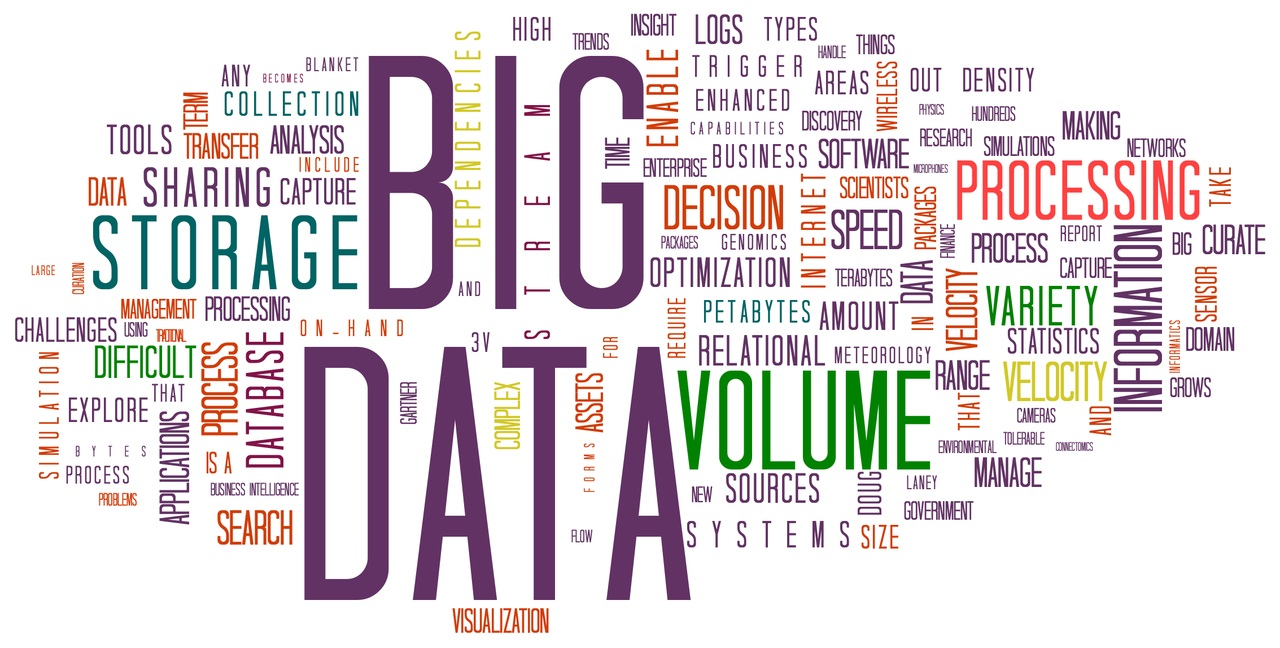
\includegraphics[scale=0.5]{BigData}
    \caption{Revista Exame 2017 (\cite{exame17})}
    %\label{figRotulo}
  \end{figure}
\end{block}
\end{frame}

\begin{frame}{}
\frametitle{Introdução}
\begin{block}{}
\justifying
\begin{itemize}
\item Google: são 3,5 bilhões de buscas por dia.\pause
\item YouTube: mais de 1 bilhão de usuários e são assistidas 100 milhões de horas de vídeos por dia.\pause
\item Facebook: 1,5 bilhões de usuários ativos em um mês.\pause
\item Instagram: 3,5 bilhões de likes e 80 milhões de fotos carregadas em um dia e 40 bilhões de fotos compartilhadas no total.\pause
\item WhatsApp: mais de 300 bilhões de mensagens por dia e 700 milhões de usuários por mês.\pause
\item Twitter: 500 milhões de tweets por dia e 316 milhões de usuários ativos por mês.
\end{itemize}
\end{block}
\end{frame}

\begin{frame}{}
\frametitle{Introdução}
\begin{block}{}
\justifying
\begin{itemize}
\item Internet: quase 950 milhões de sites e 3,2 bilhões de pessoas conectadas.\pause
\item Telefones celulares: mais de 7,5 bilhões.\pause
\item Dispositivos conectados: serão 50 bilhões em 2050.\pause
\item São gerados 2,5 exabytes ($10^{18} bytes$) de dados por dia que dobram a cada 40 meses.
\end{itemize}
\end{block}
\begin{block}{}
\justifying
A IDC (empresa líder em inteligência de mercado e consultoria nas indústrias de tecnologia da informação, telecomunicações e mercados de consumo em massa de tecnologia) estima que, do total de dados no mundo, $22\%$ contêm informação útil. E apenas $5\%$ foram analisados e utilizados de alguma forma. \cite{exame14}
\end{block}
\end{frame}

\begin{frame}{}
\frametitle{Introdução}
\begin{block}{}
\justifying
Como processar tanta informação? Como gerar informação a partir dos dados? Essa não é uma tarefa fácil, é necessário, anos de estudo e variadas competências, Estatística, Matemática, Ciência da Computação e diversas outras. Mas o profissional que tem conhecimento estatístico e sabe avaliar processos ou prever possíveis resultados de ações é um dos profissionais mais requisitados na atualidade e recebe os maiores salários!
\end{block}
\end{frame}

\begin{frame}{}
\frametitle{Introdução}
\begin{block}{Engenheiro ou Cientista de Dados}
\justifying
\begin{itemize}
\item {\bf O que faz:} combina habilidades em negócios e estatística. É o profissional responsável por solucionar problemas do negócio com técnicas de orientação a dados, bem como detectar tendências que podem ajudar nos resultados de uma empresa
\item {\bf Perfil:} qualificações estatísticas, matemáticas e curiosidade para fazer descobertas em big data
\item {\bf Salário:} R\$ 9 mil a R\$ 15 mil\\
\end{itemize}
{\bf Fonte:} \url{https://epocanegocios.globo.com/Carreira/noticia/2017/12/
profissoes-que-estarao-em-alta-no-brasil-em-2018.html}
\end{block}
\end{frame}

\begin{frame}{}
\frametitle{Introdução}
\begin{block}{}
\justifying
Você precisa ser especialista em Estatística ou Matemática ou mesmo ter feito uma graduação nestas áreas? \pause A resposta é {\bf não}. \pause Apesar dessas áreas permitirem uma compreensão mais abrangente, é possível aprender estes conceitos e aplica-los, ao longo da sua jornada de aprendizagem. Você não precisa aprender todos os tópicos relacionados à Estatística ou Matemática.

{\bf Fonte:} \url{http://datascienceacademy.com.br/blog/cientista-de-dados-por-onde-comecar-em-8-passos/}
\end{block}
\end{frame}

\begin{frame}{}
\frametitle{Introdução}
\begin{block}{}
\justifying
Estatística é a ciência que nos ajuda a tomar decisões e tirar conclusões na presença de variabilidade. A estatística é uma maneira de raciocinar que pode ajudar você a tomar decisões mais bem fundamentadas. A estatística ajuda você a solucionar problemas que envolvem decisões que estão baseadas em dados que tenham sido coletados.
\end{block}
\end{frame}

\begin{frame}{}
\frametitle{Introdução}
\begin{block}{}
\justifying
Ressalto que a Estatística é a ciência que ensina a ``ESCUTAR" os dados, não é uma ciência para provar alguma coisa em relação ao que você deseja que os dados digam!
\end{block}
\pause
\begin{block}{}
\justifying
A estatística é a arte de torturar os números até que eles confessem!
*Darrell Huff's - Como mentir com estatísticas (1954)

Leiam também \cite{super16}.
\end{block}
\end{frame}

\begin{frame}{}
\frametitle{Introdução}
\begin{block}{}
\justifying
Na primeira parte deste curso estaremos interessados em:
\begin{itemize}
\item Reduzir, Analisar e interpretar dados!
\end{itemize}
\pause
Na Análise exploratória de dados (AED) queremos obter dos dados a maior
quantidade possível de informação, para indicar modelos plausíveis a serem utilizados
na inferência estatística.
\end{block}
\end{frame}

\begin{frame}{}
\frametitle{Introdução}
\begin{block}{}
\justifying
Vamos aprender e calcular algumas medidas de posição e de variabilidade. E aprender técnicas gráficas para a análise exploratória de dados. 
\end{block}
\end{frame}

\begin{frame}{}
\frametitle{Modelos}
\begin{block}{}
\justifying
Fundamentalmente, quando se procede a uma análise de dados, busca-se alguma forma de regularidade ou padrão ou, ainda, um modelo, presente nas observações.
\end{block}
\end{frame}

\begin{frame}{}
\frametitle{Modelos}
\begin{block}{Exemplo}
\justifying
Imagine que estejamos estudando a relação entre rendimentos e gastos de consumo de um conjunto de indivíduos. Podemos obter um gráfico como o da Figura 
\ref{fig_ex1}. O que se espera, intuitivamente, é que os gastos de um indivíduo estejam diretamente relacionados com os seus rendimentos, de modo que é razoável 
supor uma “relação linear” entre essas duas quantidades. Os pontos da Figura \ref{fig_ex1} não estão todos, evidentemente, sobre uma reta, essa seria o nosso padrão 
ou modelo. A diferença entre os dados e o modelo constitui os resíduos.
\end{block}
\end{frame}

\begin{frame}{}
\frametitle{Modelos}
\begin{figure}[H]
    \centering
    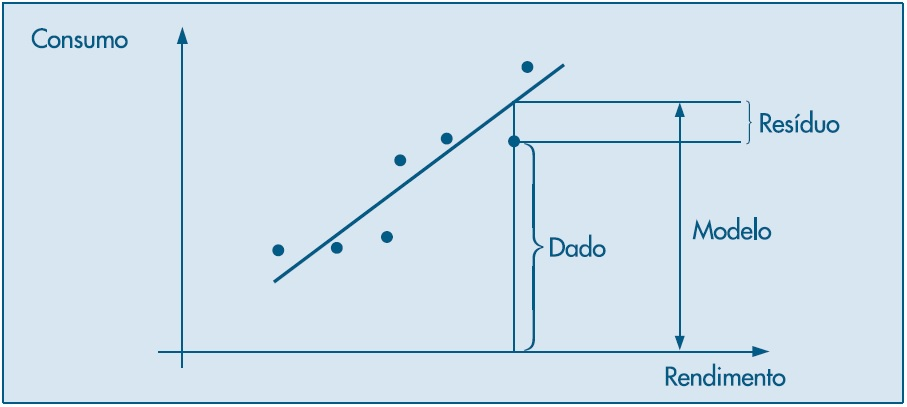
\includegraphics[scale=0.5]{Fig1}
    \caption{Relação entre consumo e rendimento (\cite{Morettin09}).}
    \label{fig_ex1}
  \end{figure}
\end{frame}

\begin{frame}{}
\frametitle{Modelos}
\begin{block}{}
\justifying
De modo esquemático:
\begin{equation}
\label{eq1}
\textrm{Dados}=\textrm{Modelo}\ +\ \textrm{Resíduos,}\quad \textrm{ou, ainda,}\quad 
D=M+R
\end{equation}
\end{block}
\pause
\begin{block}{}
\justifying
A parte M é também chamada parte suave (ou regular ou, ainda, previsível) dos dados, enquanto R é a parte aleatória. 
\end{block}
\pause
\begin{block}{}
\justifying
A parte R é tão importante quanto M, e a análise dos resíduos constitui uma parte fundamental de todo trabalho estatístico. Basicamente, são os resíduos que nos 
dizem se o modelo é adequado ou não para representar os dados.
\end{block}
\end{frame}

\begin{frame}{}
\frametitle{Modelos}
\begin{block}{}
\justifying
Uma análise exploratória de dados busca, essencialmente, fornecer informações
para estabelecer (\ref{eq1}).
\end{block}
\end{frame}

\begin{frame}{}
\frametitle{Técnicas Computacionais}
\begin{block}{}
\justifying
O desenvolvimento rápido e constante na área de computação foi acompanhado pela introdução de novas técnicas de análise de dados, notadamente de métodos 
gráficos e de métodos chamados de computação intensiva.
\end{block}
\end{frame}

\begin{frame}{}
\frametitle{Técnicas Computacionais}
\begin{block}{}
\justifying
Para a implementação dessas técnicas, foram desenvolvidos programas estatísticos, atualmente usados em larga escala tanto no meio acadêmico como em indústrias, 
bancos, órgãos de governo etc. Um dos mais utilizados na atualidade é o software R.
\end{block}
\begin{figure}[H]
    \centering
    
\includegraphics[height=0.3\textwidth, width=0.8\textwidth]{download}
    %\caption{Logo R.}
    %\label{fig_ex1}
  \end{figure}
\end{frame}

\begin{frame}{}
\frametitle{Técnicas Computacionais}
\begin{block}{}
\justifying
Por outro lado, os programas podem exigir maior ou menor experiência computacional dos usuários. Alguns operam com menus, e seu uso é mais simples. Outros 
requerem maior familiaridade com o computador e são baseados em linguagens próprias. 
\end{block}
\begin{block}{}
\textbf{Fiquem atentos}, \textbf{procurem aprender programação}, não tenha medo do computador! Estamos a bordo de uma revolução tecnológica que já está transformando 
a forma como vivemos, trabalhamos e nos relacionamos e à medida que todas as empresas se tornam digitais, a demanda por profissionais de tecnologia aumenta 
mais rápido do que a disponibilidade de mão de obra qualificada!
\end{block}
\end{frame}

\begin{frame}{}
\frametitle{Técnicas Computacionais}
\begin{block}{}
\justifying
Além dos pacotes estatísticos, há outros pacotes de grande utilidade para realizar tarefas matemáticas. Dentre estes, mencionamos o Mathematica, o Maple, o Gauss 
e o MatLab. Existe também o Wolfram Alpha e o Symbolab que é um mecanismo de conhecimento computacional que funciona on-line. Além disso, nesse curso, iremos 
utilizar o Latex como editor de texto.
\end{block}
\end{frame}

\begin{frame}{}
\frametitle{Métodos Gráficos}
\begin{block}{}
\justifying
Os métodos gráficos têm encontrado um uso cada vez maior devido ao seu forte apelo visual. Normalmente, é mais fácil para qualquer pessoa entender a mensagem 
de um gráfico do que aquela embutida em tabelas ou sumários numéricos.
\end{block}
\end{frame}

\begin{frame}{}
\frametitle{}
\begin{block}{}
\justifying
Os gráficos são utilizados para:
\begin{itemize}
\item buscar padrões e relações;\pause
\item confirmar (ou não) certas expectativas que se tinha sobre os dados;\pause
\item descobrir novos fenômenos;\pause
\item confirmar (ou não) suposições feitas sobre os procedimentos estatísticos usados; e\pause
\item apresentar resultados de modo mais rápido e fácil.
\end{itemize}
\end{block}
\end{frame}

\begin{frame}{}
\frametitle{}
\begin{block}{}
\justifying
Podemos usar métodos gráficos para plotar os dados originais ou outros dados derivados
deles. Por exemplo, a investigação da relação entre as variáveis da Figura (\ref{fig_ex1}) pode ser feita por meio daquele diagrama de dispersão. Mas podemos também “ajustar” uma reta aos dados, calcular o desvio (resíduo) para cada observação e fazer um novo gráfico, de consumo contra resíduos, para avaliar a qualidade do ajuste.
\end{block}
\end{frame}

\begin{frame}{}
\frametitle{Conjuntos de Dados}
\begin{block}{}
\justifying
Na página da disciplina (\url{https://maf105.github.io/}) aparecem alguns conjuntos de dados que serão utilizados nos exemplos ou nos exercícios propostos. Aconselho a todos a reproduzir os exemplos, usando esses dados, bem como resolver os problemas, pois somente a efetiva manipulação de dados pode levar a um bom entendimento das técnicas apresentadas.
\end{block}
\end{frame}

\begin{frame}{}
\frametitle{}
\begin{block}{}
\justifying
Os conjuntos de dados apresentados provêm de diferentes fontes, que são mencionadas
em cada conjunto e depois explicitadas nas referências. usaremos para as análises estatísticas o software R, calculadora ciêntífica e planilhas do Excel. 
\end{block}
\end{frame}

\begin{frame}{}
\frametitle{}
\begin{block}{}
\centering
{\Large \bf{Mãos à obra!!!}}
\end{block}
\end{frame}

\section{Resumo de Dados}
\begin{frame}{}
\frametitle{Tipo de Variáveis}
\begin{block}{}
\justifying
Conhecer o tipo da variável é importante porque os métodos estatísticos que você pode utilizar em sua análise variam de acordo com o tipo de variável. Existem dois 
tipos principais para variáveis:
\begin{itemize}
\item {\bf Variáveis categóricas} (ou {\bf Variáveis qualitativas}) apresentam valores que podem somente ser posicionados em categorias tais como sim e não. \pause
\item {\bf Variáveis numéricas} (ou {\bf Variáveis quantitativas}) apresentam valores que representam quantidades.
\end{itemize}
\end{block}
\end{frame}

\begin{frame}{}
\frametitle{Tipo de Variáveis}
\begin{block}{}
\justifying
Dentre as variáveis qualitativas, ainda podemos fazer uma distinção entre dois tipos: \textbf{variável qualitativa nominal}, para a qual não existe nenhuma ordenação nas
possíveis realizações, e \textbf{variável qualitativa ordinal}, para a qual existe uma ordem nos seus resultados.
\end{block}
\end{frame}

\begin{frame}{}
\frametitle{}
\begin{block}{}
\justifying
Variáveis numéricas podem ser, ainda, identificadas como \textbf{variáveis discretas} ou \textbf{variáveis contínuas}.
\end{block}
\pause
\begin{block}{}
\justifying
\textbf{Variáveis discretas} apresentam valores numéricos que surgem a partir de um processo de contagem. ``A quantidade de canais de TV a Cabo Premium que você 
assina'' é um exemplo de uma variável numérica discreta, uma vez que a resposta corresponde a um entre uma quantidade finita de números inteiros.
\end{block}
\end{frame}

\begin{frame}{}
\frametitle{}
\begin{block}{}
\justifying
Variáveis contínuas produzem respostas numéricas que surgem a partir de um processo de medição. O tempo que você espera pelo atendimento de um caixa no banco 
é um exemplo de variável numérica contínua, uma vez que a resposta pode assumir qualquer valor dentro dos limites de um continuum, ou de um intervalo.
\end{block}
\end{frame}

\begin{frame}{}
\frametitle{}
\begin{block}{}
\justifying
Em uma primeira análise, identificar o tipo da variável pode parecer fácil, embora algumas variáveis que você poderia desejar estudar possam ser categóricas ou numéricas, 
dependendo do modo como você as define. Por exemplo, ``idade'' aparentaria ser uma variável numérica evidente, mas o que acontece se você estiver interessado em 
comparar os hábitos de compra de crianças, adolescentes, pessoas de meia-idade e pessoas com idade para aposentadoria? Nesse caso, definir ``idade'' como uma 
variável categórica faria mais sentido. 
\end{block}
\end{frame}

\begin{frame}{}
\frametitle{Introdução}
\begin{block}{}
\justifying
\begin{figure}[H]
    \centering
    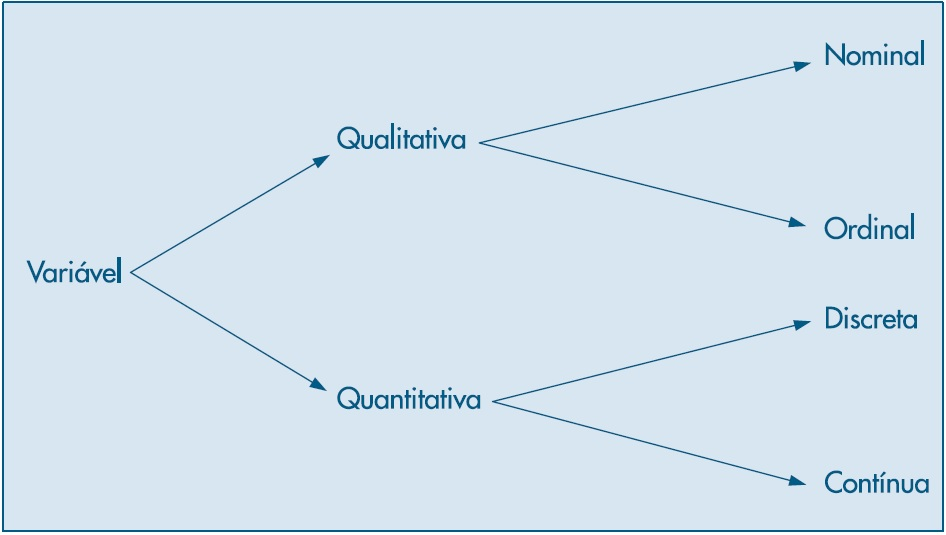
\includegraphics[scale=0.5]{Fig2}
    \caption{Classificação de uma variável (\cite{Morettin09}).}
    \label{Fig2_ex}
  \end{figure}
\end{block}
\end{frame}

\begin{frame}{}
\frametitle{Exemplo}
\begin{block}{}
\justifying
Um pesquisador está interessado em fazer um levantamento sobre alguns
aspectos socioeconômicos dos empregados da seção de orçamentos da \href{run:E:/Documentos/GitHub/MAF105/maf105.github.io/Aulas_MAF105/Aula1}{Companhia MB}. Usando informações obtidas do departamento pessoal, ele elaborou a Tabela abaixo.
\begin{table}[H]
%\caption{My caption}
\label{tab1}
\begin{tabular}{c|c}
\hline
Variável             &Representação\\
\hline
Estado Civil         &$X$\\
Grau de Instrução    &$Y$\\
Número de filhos     &$Z$\\
Salário              &$S$\\
Idade                &$U$\\
Região de Procedência&$V$\\
\hline
\end{tabular}
\end{table}
\end{block}
\end{frame}

\begin{frame}{}
\frametitle{Distribuições de Freqüências}
\begin{block}{}
\justifying
Quando se estuda uma variável, o maior interesse do pesquisador é conhecer o comportamento dessa variável, analisando a ocorrência de suas possíveis realizações. 
Vejamos uma maneira de se dispor um conjunto de realizações, para se ter uma idéia global sobre elas, ou seja, de sua distribuição.
\end{block}
\end{frame}

\begin{frame}{}
\frametitle{}
\begin{block}{}
\justifying
\begin{table}[H]
\caption{Freqüências e porcentagens dos 36 empregados da seção de orçamentos da Companhia MB segundo o grau de instrução.}
\label{tab2}
\begin{tabular}{c|c|c|c}
\hline
Grau de   &Frequência&Proporção&Porcentagem\\
instrução &$n_{i}$   &$f_{i}$  &$100f_{i}$ \\
\hline
Fundamental&12       &0,3333   &33,33      \\
Médio      &18       &0,5000   &50,00      \\
Superior   & 6       &0,1667   &16,67      \\
\hline
Total      &36       &1,0000   &100,00     \\
\hline
\end{tabular}
\end{table}
Observando os resultados da segunda coluna, vê-se que dos 36 empregados da companhia,
12 têm o ensino fundamental, 18 o ensino médio e 6 possuem curso superior.
\end{block}
\end{frame}

\begin{frame}{}
\frametitle{}
\begin{block}{}
\justifying
Uma medida bastante útil na interpretação de tabelas de freqüências é a proporção de
cada realização em relação ao total, pois podem ser utilizadas quando se quer comparar
resultados de duas pesquisas distintas.
\end{block}
\pause
\begin{block}{}
\justifying
Por exemplo, suponhamos que se queira comparar a variável grau de instrução para empregados da seção de orçamentos com a mesma variável para todos os 
empregados da Companhia MB. Digamos que a empresa tenha 2.000 empregados e que a distribuição de frequências seja a da próxima Tabela.
\end{block}
\end{frame}

\begin{frame}{}
\frametitle{}
\begin{block}{}
\justifying
\begin{table}[H]
\caption{Freqüências e porcentagens dos dos 2.000 empregados da Companhia MB segundo o grau de instrução.}
\label{tab3}
\begin{tabular}{c|c|c|c}
\hline
Grau de   &Frequência&Proporção&Porcentagem\\
instrução &$n_{i}$   &$f_{i}$  &$100f_{i}$ \\
\hline
Fundamental&650      &0.325    &32.50      \\
Médio      &1.020    &0.51     &51.00      \\
Superior   & 330     &0.165    &16.50      \\
\hline
Total      &2.000    &1,0000   &100.00     \\
\hline
\end{tabular}
\end{table}
Não podemos comparar diretamente as colunas das frequências das Tabelas \ref{tab2} e \ref{tab3}, pois os totais de empregados são diferentes nos dois casos. Mas 
as colunas das porcentagens são comparáveis, pois reduzimos as frequências a um mesmo total (no caso 100).
\end{block}
\end{frame}

\begin{frame}{}
\frametitle{}
\begin{block}{}
\justifying
A construção de tabelas de frequências para variáveis contínuas necessita de certo
cuidado. Por exemplo, a construção da tabela de frequências para a variável salário,
usando o mesmo procedimento acima, \textbf{não resumirá as 36 observações} num grupo
menor, pois não existem observações iguais. A solução empregada é agrupar os dados
por faixas de salário.
\end{block}
\end{frame}

\begin{frame}{}
\frametitle{}
\begin{block}{}
\justifying
\begin{table}[H]
\caption{Frequências e porcentagens dos dos 2.000 empregados da seção de orçamentos da Companhia MB por faixa de salário.}
\label{tab4}
\begin{tabular}{c|c|c}
\hline
Classe de   &Frequência&Porcentagem\\
Salários    &$n_{i}$   &$100f_{i}$ \\
\hline
4.00|-8.00  &10        &27.78      \\
8.00|-12.00 &12        &33.33      \\
12.00|-16.00&8         &22.22      \\
16.00|-20.00&5         &13.89      \\
20.00|-24.00&1         & 2.78      \\
\hline
Total       &36        &100.00     \\
\hline
\end{tabular}
\end{table}
\end{block}
\end{frame}

\begin{frame}{}
\frametitle{}
\begin{block}{}
\justifying
Procedendo-se desse modo, ao resumir os dados referentes a uma variável contínua,
perde-se alguma informação. Por exemplo, não sabemos quais são os oito salários da
classe de 12 a 16, a não ser que investiguemos a tabela original. Sem perda de muita precisão, poderíamos supor que todos os oito salários daquela classe fossem iguais ao ponto médio da referida classe, isto é, 14.
\end{block}
\end{frame}

\begin{frame}{}
\frametitle{}
\begin{block}{}
\justifying
Note que estamos usando a notação $a|-b$ para o intervalo de números contendo o extremo $a$ mas não contendo o extremo $b.$ Podemos também usar a notação $[a, b)$ para designar o mesmo intervalo $a|-b$. 
\end{block}
\end{frame}

\begin{frame}{}
\frametitle{}
\begin{block}{}
\justifying
A escolha dos intervalos é arbitrária e a familiaridade do pesquisador com os dados é
que lhe indicará quantas e quais classes (intervalos) devem ser usadas.
\begin{itemize}
\item Número pequeno de classes $\rightarrow$ perda de informação;\pause
\item Número grande de classes $\rightarrow$ perda da visão geral dos dados
como um conjunto;\pause
\item A sugestão é usar de 5 a 15 classes com a mesma amplitude;
\end{itemize}
\end{block}
\end{frame}

\begin{frame}{}
\frametitle{}
\begin{block}{}
\justifying
Para construir uma distribuição de frequências separando por classes uma determinada variável podemos utilizar:
\begin{itemize}
\item número de classes($n_{c}$)$\approx \sqrt{n}$ ou usamos a regra de Sturges $n_{c}=\ln{(n)};$\pause
\item Amplitude da classe $=\dfrac{AT}{n_{c}}$ 
\end{itemize}
em que $AT=\textrm{Maior valor} - \textrm{Menor valor}.$
\end{block}
\end{frame}

\begin{frame}{}
\frametitle{}
\begin{block}{}
\justifying
Um procedimento alternativo para resumir um conjunto de valores, com o objetivo de se
obter uma idéia da forma de sua distribuição, é o ramo-e-folhas. Uma vantagem deste diagrama é que não perdemos (ou perdemos pouca) informação sobre os dados em si.
\end{block}
\end{frame}

\begin{frame}{}
\frametitle{Diagrama de ramos e folhas para variáveis contínuas}
\begin{block}{}
\justifying
Quando o número de observações é relativamente grande, este diagrama pode ser útil.
\begin{table}[H]
\caption{Diagrama de Ramos e Folhas da idade}
\begin{tabular}{c|ccccccccccccccccc}
Ramo&\multicolumn{17}{c}{Folhas}\\
\hline
2&0&3&5&6&6&7&8&9& & & & & & & & & \\
3&0&1&1&2&2&3&3&4&4&5&5&6&6&7&7&8&9\\
4&0&0&1&1&2&3&3&4&6&8& & & & & & & 
\end{tabular}
\end{table}
\end{block}
\end{frame}

\begin{frame}{}
\frametitle{}
\begin{block}{}
\justifying
\begin{table}[H]
\caption{Diagrama de Ramos e Folhas dos Salários ($\times$ sal. Min)}
\scalebox{0.6}{%
\begin{tabular}{c|cccccccc}
Ramo&\multicolumn{8}{c}{Folhas}\\
\hline
 4&& 00&& 56&&   &&   \\
 5&& 25&& 73&&   &&   \\
 6&& 26&& 66&& 86&&   \\
 7&& 39&& 44&& 59&&   \\
 8&& 12&& 46&& 74&& 95\\
 9&& 13&& 35&& 77&& 80\\
10&& 53&& 76&&   &&   \\
11&& 06&& 59&&   &&   \\
12&& 00&& 79&&   &&   \\
13&& 23&& 60&& 85&&   \\
14&& 69&& 71&&   &&   \\
15&& 99&&   &&   &&   \\
16&& 22&&   && 61&&   \\
17&& 26&&   &&   &&   \\
18&& 75&&   &&   &&   \\
19&& 40&&   &&   &&   \\
20&&   &&   &&   &&   \\
21&&   &&   &&   &&   \\
22&&   &&   &&   &&   \\
23&&   && 30&&   &&   \\
\end{tabular}}
\end{table}
\end{block}
\end{frame}

\begin{frame}{}
\frametitle{}
\begin{block}{}
\justifying
Algumas informações que se obtêm deste ramo-e-folhas são:
\begin{enumerate}
\item Há um destaque grande para o valor 23,30.\pause
\item Os demais valores estão razoavelmente concentrados entre 4,00 e 19,40.\pause
\item Um valor mais ou menos típico para este conjunto de dados poderia ser, por 
exemplo, 10,00.\pause
\item Há uma leve assimetria em direção aos valores grandes; a suposição de que estes dados possam ser considerados como amostra de uma população com distribuição simétrica, em forma de sino (a chamada distribuição normal), pode ser questionada.
\end{enumerate}
\end{block}
\end{frame}

\section{Representação gráfica}
\begin{frame}{}
\frametitle{}
\begin{block}{}
\justifying
A representação gráfica da distribuição de uma variável tem a vantagem de, rápida e concisamente, informar sobre sua variabilidade. Existem vários gráficos que podem ser utilizados. Vejamos alguns!
\end{block}
\end{frame}

\begin{frame}{}
\frametitle{Gráficos para Variáveis Qualitativas}
\begin{block}{}
\justifying
Existem vários tipos de gráficos para representar variáveis qualitativas. Vários são
versões diferentes do mesmo princípio, logo nos limitaremos a apresentar dois deles:
gráficos em barras e de composição em setores (“pizza” ou retângulos).
\end{block}
\end{frame}

\begin{frame}{}
\frametitle{}
\begin{block}{}
\justifying
Tomemos como ilustração a variável Y: grau de instrução, exemplificada
nas Tabelas 2.2 e 2.3. O gráfico em barras consiste em construir retângulos ou barras,
em que uma das dimensões é proporcional à magnitude a ser representada $(n_{i}\ \textrm{ou}\ f_{i}),$ sendo a outra arbitrária, porém igual para todas as barras. Essas barras são dispostas paralelamente umas às outras, horizontal ou verticalmente. Na próxima Figura temos o gráfico em barras (verticais) para a variável $Y.$
\end{block}
\end{frame}

\begin{frame}{}
\frametitle{}
\begin{block}{}
\justifying
\begin{figure}[H]
    \centering
    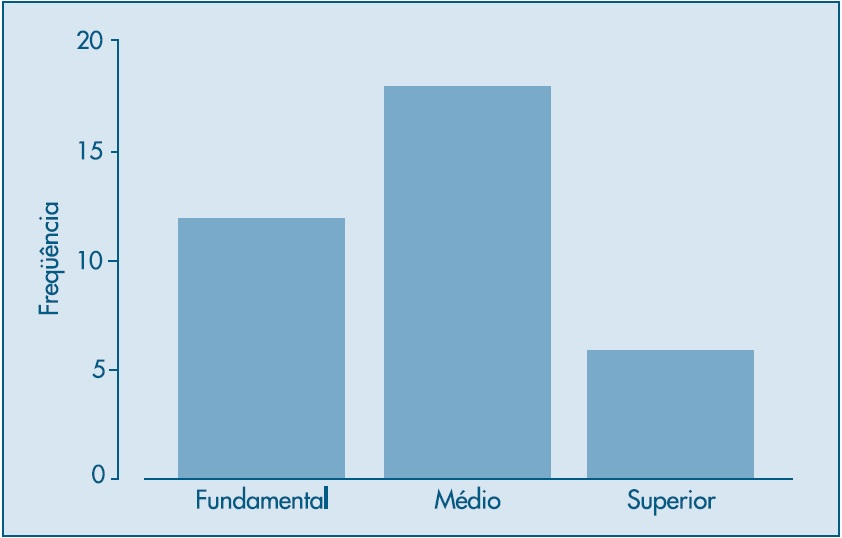
\includegraphics[scale=0.5]{Fig3}
    \caption{Gráfico em barras para a variável $Y:$ grau de instrução (\cite{Morettin09}).}
    \label{Fig3_ex}
  \end{figure}
\end{block}
\end{frame}

\begin{frame}{}
\frametitle{}
\begin{block}{}
\justifying
Já o gráfico de composição em setores, sendo em forma de “pizza” o mais conhecido,
destina-se a representar a composição, usualmente em porcentagem, de partes de um todo.
Consiste num círculo de raio arbitrário, representando o todo, dividido em setores, que
correspondem às partes de maneira proporcional. A próxima Figura mostra esse tipo de gráfico para a variável $Y.$
\end{block}
\end{frame}

\begin{frame}{}
\frametitle{}
\begin{block}{}
\justifying
\begin{figure}[H]
    \centering
    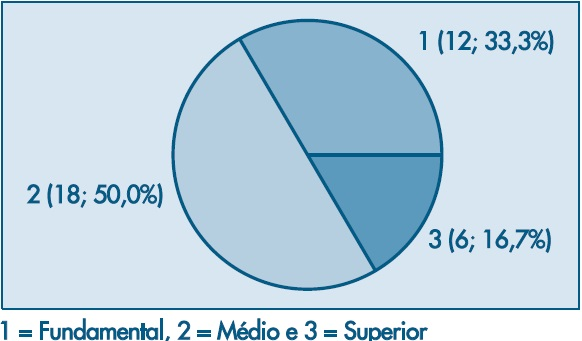
\includegraphics[scale=0.5]{Fig4}
    \caption{Gráfico em setores para a variável $Y:$ grau de instrução (\cite{Morettin09}).}
    \label{Fig4_ex}
  \end{figure}
\end{block}
\end{frame}

\begin{frame}{}
\frametitle{Gráficos para Variáveis Quantitativas}
\begin{block}{}
\justifying
Para variáveis quantitativas podemos considerar uma variedade maior de representações
gráficas. Podemos considerar gráficos de barra, gráfico de pontos, gráficos com barras 
empilhadas, gráficos de dispersão e outros. Mas para resumir os dados, o mais utilizado 
é o histograma.
\end{block}
\end{frame}

\begin{frame}{}
\frametitle{}
\begin{block}{}
\justifying
O histograma é um gráfico de barras contíguas, com as bases proporcionais aos intervalos
das classes e a área de cada retângulo proporcional à respectiva frequência. Pode-se
usar tanto a frequência absoluta, $f_{i},$ como a relativa, $f_{ri}.$
\end{block}
\end{frame}

\begin{frame}{}
\frametitle{}
\begin{block}{}
\justifying
\begin{figure}[H]
    \centering
    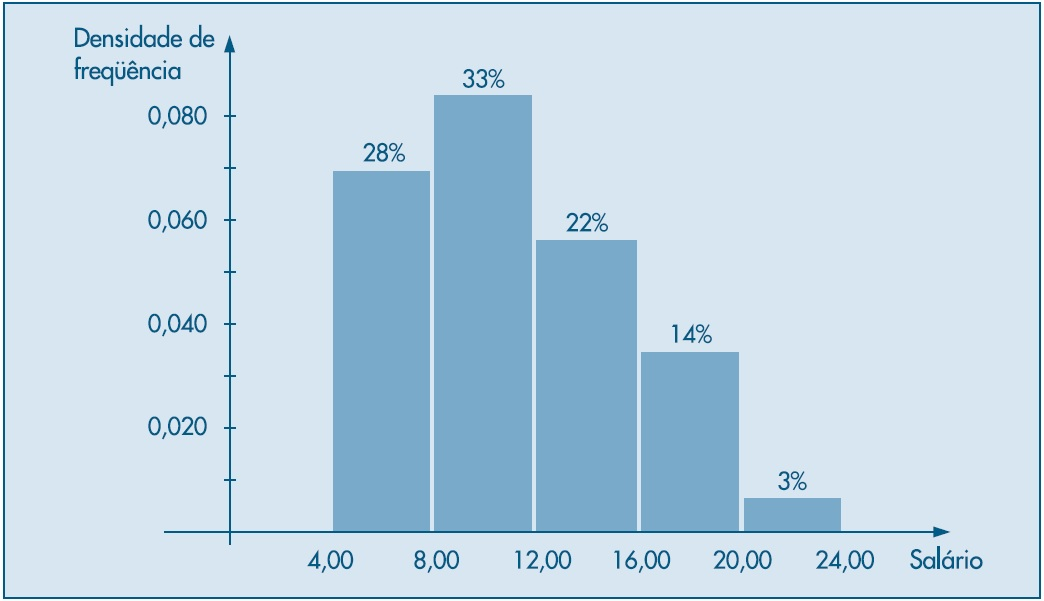
\includegraphics[scale=0.5]{Fig5}
    \caption{Histograma da variável $S:$ Salários (\cite{Morettin09}).}
    \label{Fig5_ex}
  \end{figure}
\end{block}
\end{frame}

\begin{frame}{}
\frametitle{}
\begin{block}{}
\justifying
Para facilitar o entendimento, foi colocada acima de cada setor (retângulo) a respectiva
porcentagem das observações (arredondada). Assim, por meio da figura, podemos
dizer que $61\%$ dos empregados têm salário inferior a 12 salários mínimos, ou
$17\%$ possuem salário superior a 16 salários mínimos.
\end{block}
\end{frame}

\begin{frame}{}
\frametitle{}
\begin{block}{}
\justifying
Do mesmo modo que usamos um artifício para representar uma variável contínua
como uma variável discreta, podemos usar um artifício para construir um histograma
para variáveis discretas. A próxima Figura é um exemplo de como ficaria o histograma da
variável $Z,$ número de filhos dos empregados casados.
\end{block}
\end{frame}

\begin{frame}{}
\frametitle{}
\begin{block}{}
\justifying
\begin{figure}[H]
    \centering
    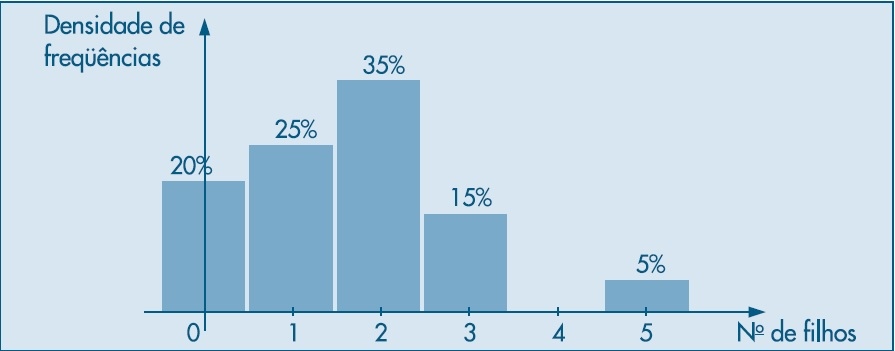
\includegraphics[scale=0.5]{Fig6}
    \caption{Histograma da variável $Z:$ número de filhos (\cite{Morettin09}).}
    \label{Fig6_ex}
  \end{figure}
\end{block}
\end{frame}


\begin{frame}{}
\frametitle{}
\begin{block}{}
\justifying
Caso utilizemos as frequências acumuladas ou frequências acumuladas relativas para construir o histograma teríamos um histograma conhecido como {\bf ogiva} ou {\bf ogiva percentual}, respectivamente.
\end{block}
\end{frame}

\section{Medidas de Posição}
\begin{frame}{}
\frametitle{}
\begin{block}{}
\justifying
Vimos que o resumo de dados por meio de tabelas de frequências e ramo-e-folhas fornece
muito mais informações sobre o comportamento de uma variável do que a própria tabela
original de dados. 
\end{block}
\pause
\begin{block}{}
\justifying
Muitas vezes, queremos resumir ainda mais estes dados, apresentando um ou alguns valores que sejam representativos da série toda. \textbf{Quando usamos um só 
valor, obtemos uma redução drástica dos dados.} Usualmente, emprega-se uma das seguintes medidas de posição (ou localização) central: média, mediana ou moda.
\end{block}
\end{frame}

\begin{frame}{}
\frametitle{}
\begin{block}{}
\justifying
A moda é definida como a realização mais frequente do conjunto de valores observados. Por exemplo, considere a variável $Z,$ número de filhos de cada funcionário 
casado, resumida na Tabela de dados da companhia MB. Vemos que a moda é 2, correspondente à realização com maior frequência, 7. Em alguns casos, pode haver 
mais de uma moda, ou seja, a distribuição dos valores pode ser bimodal, trimodal etc.
\end{block}
\end{frame}

\begin{frame}{}
\frametitle{}
\begin{block}{}
\justifying
A mediana é a realização que ocupa a posição central da série de observações, quando
estão ordenadas em ordem crescente. Assim, se as cinco observações de uma variável forem $3, 4, 7, 8$ e $8,$ a mediana é o valor $7,$ correspondendo à terceira 
observação. Quando o número de observações for par, usa-se como mediana a média aritmética das duas observações centrais. Acrescentando-se o valor $9$ à série acima, a mediana será $(7 + 8)/2 = 7,5.$
\end{block}
\end{frame}

\begin{frame}{}
\frametitle{}
\begin{block}{}
\justifying
Finalmente, a média aritmética, conceito familiar ao leitor, é a soma das observações dividida pelo número delas.
\end{block}
\end{frame}

%\begin{frame}{}
%\frametitle{}
%\begin{block}{}
%\justifying
%Neste exemplo, as três medidas têm valores próximos e qualquer uma delas pode ser
%usada como representativa da série toda. A média aritmética é, talvez, a medida mais usada.
%Contudo, ela pode conduzir a erros de interpretação. Em muitas situações, a mediana é uma
%medida mais adequada. Veremos algumas situações que ilustram tal afirmação.
%\end{block}
%\end{frame}

\begin{frame}{}
\frametitle{}
\begin{block}{}
\justifying
Se $x_{1},\cdots,x_{n}$ são os $n$ valores (distintos ou não) da variável $X,$ a média aritmética, ou simplesmente média, de $X$ pode ser escrita como:
\begin{equation}
\bx=\dfrac{x_{1}+\cdots+x_{n}}{n}=\dfrac{\displaystyle \sum_{i=1}^{n}{x_{i}}}{n}
\end{equation}
Agora, se tivermos $n$ observações da variável $X,$ das quais $n_{1}$ são iguais a $x_{1},$ $n_{2}$ são iguais
a $x_{2},$ $n_{k}$ iguais a $x_{k},$ então a média de $X$ pode ser escrita como:
\begin{equation}
\bx=\dfrac{n_{1}x_{1}+\cdots+n_{k}x_{k}}{n}=\dfrac{\displaystyle \sum_{i=1}^{k}n_{i}x_{i}}{n}
\end{equation}
\end{block}
\end{frame}

\begin{frame}{}
\frametitle{}
\begin{block}{}
\justifying
Consideremos, agora, as observações ordenadas em ordem crescente. Vamos denotar a
menor observação por $x_{(1)},$ a segunda por $x_{(2)},$ e assim por diante, obtendo-se
\begin{equation}\label{est_ordem}
x_{(1)}\leq x_{(2)}\leq \cdots \leq x_{(n-1)}\leq x_{(n)}.
\end{equation}
As observações ordenadas como em (\ref{est_ordem}) são chamadas {\bf estatísticas de ordem}. Com esta notação, a mediana da variável $X$ pode ser definida como:
\[
md(X)=\left\{
\setlength\arraycolsep{0pt}
\begin{array}{lr}
X_{(\frac{n+1}{2})},                                             &\quad \textrm{se}\quad $n$\quad \textrm{é impar,}\\
&\\
\frac{X_{(\frac{n}{2})}+X_{(\frac{n}{2}+1)}}{2},  &\quad \textrm{se}\quad $n$\quad \textrm{é par.}\\
\end{array}
\right.
\]
\end{block}
\end{frame}

\begin{frame}{}
\frametitle{}
\begin{block}{}
\justifying
A mediana é uma medida mais robusta que a média, quando submetida a mudanças nos valores observados, ou a incorporação de mais observações no conjunto de dados original.
\end{block}
\end{frame}

\section{Medidas de Dispersão}
\begin{frame}{}
\frametitle{}
\begin{block}{}
\justifying
O resumo de um conjunto de dados por uma única medida representativa de posição
central esconde toda a informação sobre a variabilidade do conjunto de observações.
Por exemplo, suponhamos que cinco grupos de alunos submeteram-se a um
teste, obtendo-se as seguintes notas:
\begin{itemize}
\item Grupo A (Variável $X$): 3,4,5,6,7
\item Grupo B (Variável $Y$): 1,3,5,7,9
\item Grupo C (Variável $Z$): 5,5,5,5,5
\item Grupo D (Variável $W$): 3,5,5,7
\item Grupo E (Variável $V$): 3,5,5,6,6
\end{itemize}
\end{block}
\end{frame}

\begin{frame}{}
\frametitle{}
\begin{block}{}
\justifying
Vemos que $\bar{x}=\bar{y}=\bar{z}=\bar{w}=\bar{v}=5$. A identificação de cada uma destas séries por sua
média (5, em todos os casos) nada informa sobre suas diferentes variabilidades. Notamos, então, a conveniência de serem criadas medidas que sumarizem a variabilidade de um conjunto de observações e que nos permita, por exemplo, comparar conjuntos diferentes de valores, como os dados acima, segundo algum critério estabelecido.
\end{block}
\end{frame}

%\begin{frame}{}
%\frametitle{}
%\begin{block}{}
%\justifying
%Um critério freqüentemente usado para tal fim é aquele que mede a dispersão dos
%dados em torno de sua média, e duas medidas são as mais usadas: desvio médio e variância.
%O princípio básico é analisar os desvios das observações em relação à média dessas
%observações.
%\end{block}
%\end{frame}

\begin{frame}{}
\frametitle{}
\begin{block}{}
\justifying
Um critério frequentemente usado para tal fim é aquele que mede a dispersão dos
dados em torno de sua média, e duas medidas são as mais usadas: desvio médio e variância.
\begin{align}
Dm(X) &=\displaystyle \dfrac{\sum_{i=1}^{n}|x_{i}-\bar{x}|}{n}\\
Var(X)&=\displaystyle \dfrac{\sum_{i=1}^{n}(x_{i}-\bar{x})^{2}}{n}
\end{align}
O princípio básico é analisar os desvios das observações em relação à média dessas observações. Desvio é interpretado como o afastamento de uma observação em relação a uma determinada medida de posição.
\end{block}
\end{frame}

\begin{frame}{}
\frametitle{}
\begin{block}{}
\justifying
Sendo a variância uma medida de dimensão igual ao quadrado da dimensão dos dados (por exemplo, se os dados são expressos em $cm,$ a variância será expressa 
em $cm^{2}$), ela pode causar problemas de interpretação. Costuma-se usar, então, o desvio padrão, que é definido como a raiz quadrada positiva da variância.
\begin{equation}
dp(X)=\sqrt{Var(X)}
\end{equation}
Ambas as medidas de dispersão ($Dm$ e $dp$) indicam em média qual será o ``erro'' (desvio) cometido ao tentar substituir cada observação pela medida resumo do 
conjunto de dados (no caso, a média).
\end{block}
\end{frame}

\begin{frame}{}
\frametitle{Coeficiente de Variação}
\begin{block}{}
\justifying
\begin{equation}
CV(X)=\dfrac{dp(X)}{\bar{X}}
\end{equation}
Mesmo o DP pode induzir à conclusões errôneas com relação à variabilidade. Suponha dois conjunto de dados 
$D_{1}=\{10,20,30\}$ e $D_{2}=\{10000,10010,10020\}.$ Note que nestes casos $\bar{x}_{1}=20, dp(x)=10, 
\bar{x}_{2}=10010$ e $dp(x_{2})=10.$ Porém, em termos percentuais, o primeiro conjunto de dados é mais 
heterogênio.
\end{block}
\end{frame}

\section{Medidas Complementares}
\begin{frame}{}
\frametitle{Medidas Complementares para Análise de Dados}
\begin{block}{}
\justifying
\begin{itemize}
\item Extremos: O menor e o maior valor do conjunto de dados;
\item Quartis (Q)
\begin{itemize}
\item $1^{\circ}$ Quartil: deixa um quarto dos valores abaixo, e três quartos acima dele;
\item $2^{\circ}$ Quartil $=$ Mediana: deixa metade dos valores abaixo, e metade acima dele;
\item $3^{\circ}$ Quartil: deixa três quartos dos valores abaixo, e um quarto acima dele;
\end{itemize}
\item Intervalo Interquartil (pode ser considerada uma medida robusta de dispersão).
\end{itemize}
\end{block}
\end{frame}

\begin{frame}{}
\frametitle{Distância Interquartil}
\begin{block}{}
\justifying
Uma medida de dispersão alternativa ao desvio padrão é a distância interquartil, definida como a diferença entre o terceiro e primeiro quartis, ou seja:
$$d_{q}=q_{3}-q_{1}$$
\end{block}
\end{frame}

\begin{frame}{}
\frametitle{Cálculo dos Quartis}
\begin{block}{}
\justifying
Seja $n$ o número total de elementos da amostra e calcule $\dfrac{j(n+1)}{4},$ para $j=1,2$ e $3$. Desta forma $q_{j}$ será um elemento entre $X_{k}$ e $X_{k+1},$ onde $k$ é o maior inteiro menor ou igual a 
$\dfrac{j(n+1)}{4}$ e será calculado da seguinte forma:
\begin{equation}
q_{j}=X_{k}+\Biggl(\dfrac{j(n-1)}{4}-k\Biggl)(X_{k+1}-X_{k})
\end{equation}

Podemos observar que quando $k$ é um valor inteiro, o quantil será o próprio $X_{k}$, isto é, $q_{j}=X_{k}$, onde 
$k=\dfrac{j(n+1)}{4}, j=1,2,3$.

\end{block}
\end{frame}

\begin{frame}{}
\frametitle{}
\begin{block}{}
\justifying
Os cinco valores, $x(1), q_{1}, q_{2}, q_{3} e x(n)$ são importantes para se ter uma boa ideia da assimetria da distribuição dos dados. Para uma distribuição simétrica 
ou aproximadamente simétrica, deveríamos ter:
\begin{enumerate}
\item[(a)] $q_{2}-x_{(1)}\approx x_{(n)}-q_{2};$
\item[(b)] $q_{2}-q_{(1)}\approx q_{(3)}-q_{2};$
\item[(c)] $q_{1}-x_{(1)}\approx x_{(n)}-q_{3};$
\item[(d)] distâncias entre mediana e $q_{1}, q_{3}$ menores do que distâncias entre os extremos e $q_{1}, q_{3}.$
\end{enumerate}
\end{block}
\end{frame}

\begin{frame}{}
\frametitle{}
\begin{block}{}
\justifying
A diferença $q_{2}- x_{(1)}$ é chamada dispersão inferior e $x_{(n)}-q_{2}$ é a dispersão superior.
A condição (a) nos diz que estas duas dispersões devem ser aproximadamente iguais, para uma distribuição 
aproximadamente simétrica. A próxima Figura ilustra estes fatos para a chamada distribuição normal ou gaussiana.
\end{block}
\end{frame}

\begin{frame}{}
\frametitle{}
\begin{block}{}
\justifying
\begin{figure}[H]
    \centering
    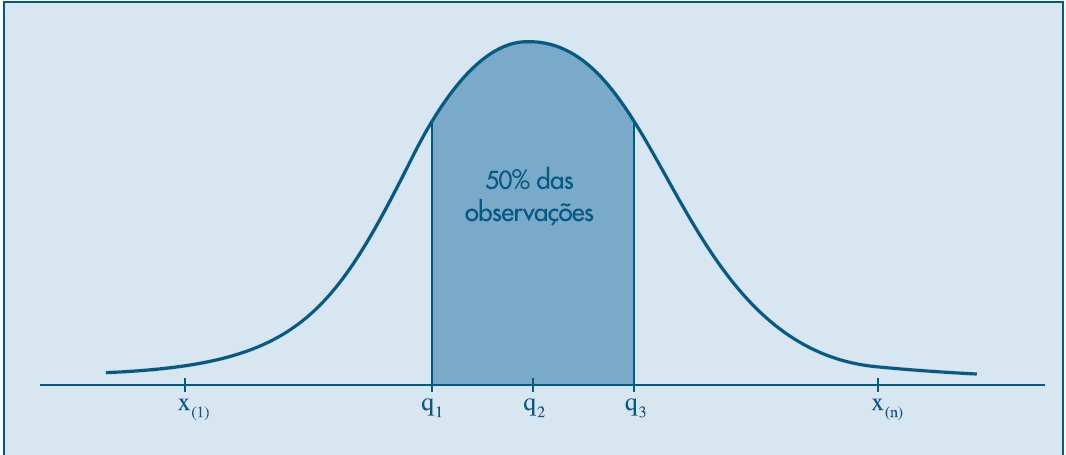
\includegraphics[scale=0.5]{Fig7}
    \caption{Uma distribuição simétrica: normal ou gaussiana (\cite{Morettin09}).}
    \label{Fig7_ex}
  \end{figure}
\end{block}
\end{frame}

\begin{frame}{}
\frametitle{}
\begin{block}{}
\justifying
As cinco estatísticas de ordem consideradas acima podem ser representadas esquematicamente como na próxima Figura, onde também incorporamos o número de 
observações, $n.$ Representamos a mediana por $md,$ os quartis por $q$ e os extremos por $E.$
\begin{figure}[H]
    \centering
    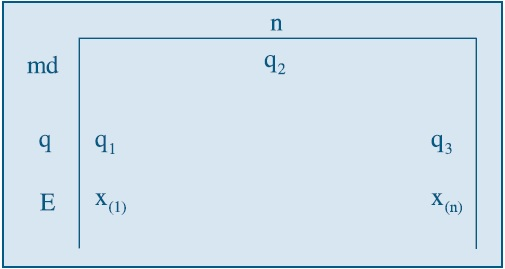
\includegraphics[scale=0.5]{Fig8}
    \caption{Esquema dos cinco números (\cite{Morettin09}).}
    \label{Fig8_ex}
  \end{figure}
\end{block}
\end{frame}

\begin{frame}{}
\frametitle{}
\begin{block}{}
\begin{figure}
\centering
\begin{tikzpicture}[xscale=1.5, yscale=7, declare function={stdnorm(\x) = 1/(sqrt(2*pi))*exp(-0.5*(pow(\x,2)));}]
\fill[gray] (-2.5,0) -- plot [domain=-2.5:-3/2, samples=50] (\x, {stdnorm(\x)}) -- (-3/2,0) -- cycle;
\fill[gray] (3/2,0) -- plot [domain=3/2:5/2, samples=50] (\x, {stdnorm(\x)}) -- (5/2,0) -- cycle;
\draw [thick, domain=-2.5:2.5, samples=50] plot (\x, {stdnorm(\x)});
\draw [->] (-3,0) -- (3,0) ;
\node [below right] at (3,0) {$z$} ;
\draw [dashed] (0,0) -- (0,{stdnorm(0)}) ;
\draw [dashed] (-3/2,0) -- (-3/2,{stdnorm(-3/2)}) ;
\draw [dashed] (3/2,0) -- (3/2,{stdnorm(3/2)}) ;
\node [below] at (0,0) {$0$};
\node [below] at (-3/2,0) {$-1.96$};
\node [below] at (3/2,0) {$1.96$};
\node [above] at (-2.5,0.1) {\small{RR$\Ho$}};
\node [above] at (2.5,0.1) {\small{RR$\Ho$}};
\node [above] at (-1,0.5) {\small{RNR$\Ho$}};
\node [above] at (2,0.5) {$z_{cal}=3.25$};
\node [above] at (2,0.4) {p-valor$=0.0012$};
\node [above] at (2,0.3) {$\alpha=0.05$};
%\draw[->] (-2.7,0.15) .. controls (.-2,.2) .. (-1.9, 0.03);
\draw[->] (-2.2,0.15) to [out=20,in=90] (-1.9,0.02);
\draw[->] (2.2,0.15) to [out=160,in=90] (1.9,0.02);
\draw[->] (-0.6,0.55) to [out=0,in=90] (0.1,0.3);
%\draw [->,thick] (2.7,0.15) to [out=120,in=0] (2.3,0.3)
%to [out=0,in=90] (1.9,0.03);
%\draw (0,0) .. controls (0,4) and (4,0) .. (4,4)
%\draw[->] ( 3,0.15) .. controls (. 30,.2) .. (1.9, 0.03);
%\node at (1.8,{stdnorm(2.3)}) {\small{$\alpha/2$}};
%\node at (-1.8,{stdnorm(2.3)}){\small{$\alpha/2$}};
\end{tikzpicture}
%\caption{Região crítica para $\Ho: \mu = 50$ versus $\Hi: \mu \neq 50$ e $n = 25$}
\end{figure}
\end{block}
\end{frame}

\begin{frame}{}
\frametitle{Box-Plot}
\begin{block}{}
\justifying
\begin{figure}[H]
    \centering
    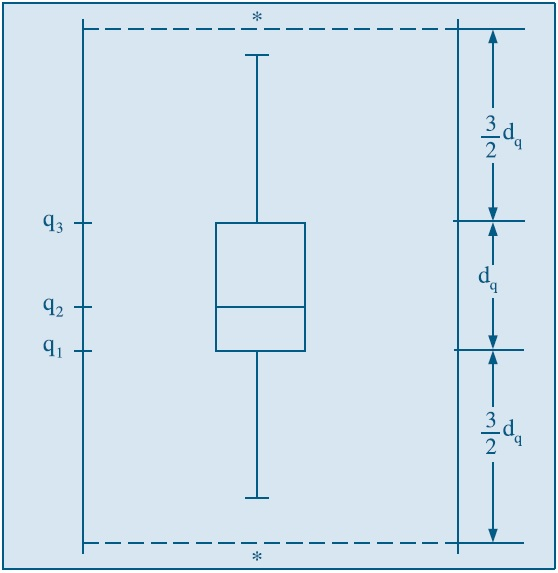
\includegraphics[height=0.4\textwidth]{Fig9}
    \caption{Esquema de um BoxPlot (\cite{Morettin09}).}
    \label{Fig9_ex}
  \end{figure}
\end{block}
\end{frame}

\begin{frame}{}
\frametitle{Box-Plot}
\begin{block}{}
\justifying
O boxplot (gráfico de caixa) é um gráfico utilizado para avaliar a distribuição empírica do dados. O boxplot é formado pelo primeiro e terceiro quartil e pela mediana. Para construir este diagrama, consideremos um retângulo onde estão representados a mediana e os quartis. A partir do retângulo, para cima, segue uma linha até o ponto mais remoto que não exceda $LS = q_{3} + (1,5)d_{q},$ chamado limite superior. De modo similar, da parte inferior do retângulo, para baixo, segue uma linha até o ponto mais remoto que não seja menor do que 
$LI = q_{1}-(1,5)d_{q},$ chamado limite inferior.
\end{block}
\end{frame}

\begin{frame}{}
\frametitle{Box-Plot}
\begin{block}{}
\justifying
Os valores compreendidos entre esses dois limites são chamados valores adjacentes. As observações que estiverem acima do limite superior ou abaixo do limite inferior estabelecidos serão chamadas pontos exteriores e representadas por asteriscos. Essas são observações destoantes das demais e
podem ou não ser o que chamamos de outliers ou valores atípicos.
\end{block}
\end{frame}

\begin{frame}{}
\frametitle{}
\begin{block}{}
\justifying
O box plot dá uma idéia da posição, dispersão, assimetria, caudas e dados discrepantes.
A posição central é dada pela mediana e a dispersão por $d_{q}.$ As posições relativas de $q_{1}, q_{2}, q_{3}$
dão uma noção da assimetria da distribuição. Os comprimentos das caudas são dados pelas
linhas que vão do retângulo aos valores remotos e pelos valores atípicos.
\end{block}
\end{frame}

\section{Assimetrias e Transformações}
\begin{frame}{}
\frametitle{Assimetrias}
\begin{figure}[H]
    \centering
    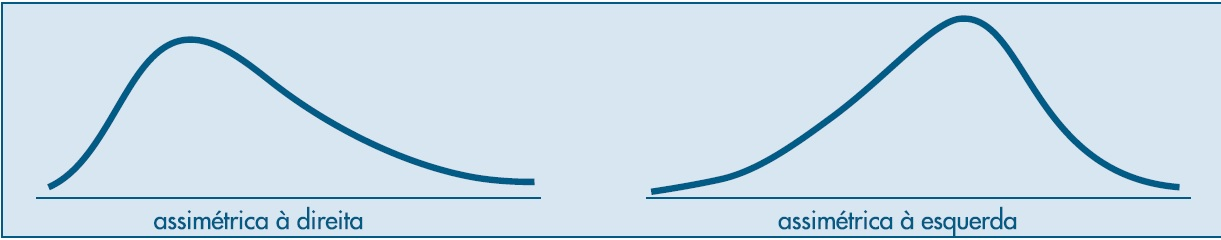
\includegraphics[height=0.4\textwidth,width=15cm]{Fig10}
    \caption{Distribuições assimétricas (\cite{Morettin09}).}
    \label{Fig10_ex}
  \end{figure}
\end{frame}

\begin{frame}{}
\frametitle{Transformações}
\begin{block}{}
\justifying
Vários procedimentos estatísticos são baseados na suposição de que os dados provêm
de uma distribuição normal (em forma de sino) ou então mais ou menos simétrica.
Mas, em muitas situações de interesse prático, a distribuição dos dados da amostra
é assimétrica e pode conter valores atípicos, como vimos em exemplos anteriores.
\end{block}
\end{frame}

\begin{frame}{}
\frametitle{}
\begin{block}{}
\justifying
Se quisermos utilizar tais procedimentos, o que se propõe é efetuar uma transformação
das observações, de modo a se obter uma distribuição mais simétrica e próxima
da normal. Uma família de transformações frequentemente utilizada é
\[
X^{*}=\left\{
\setlength\arraycolsep{0pt}
\begin{array}{lr}
X^{p},                              &\quad \textrm{se}\quad $p>0$\\
&\\
\ln{(X)},                           &\quad \textrm{se}\quad $p=0$\\
&\\
-X^{p},                             &\quad \textrm{se}\quad $p<0$\\
\end{array}
\right.
\]
Normalmente, o que se faz é experimentar valores de $p$ na sequência 
$\cdots, -3, -2, -1, -1/2, -1/3, -1/4, 0, 1/4, 1/3, 1/2, 1, 2, 3,\cdots$
\end{block}
\end{frame}

\begin{frame}{}
\frametitle{}
\begin{block}{}
\justifying
Para cada valor de $p$ obtemos gráficos apropriados (histogramas, desenhos esquemáticos etc.)
para os dados originais e transformados, de modo a escolhermos o valor mais adequado de p. Para dados positivos, 
a distribuição dos dados é usualmente assimétrica à direita. Para essas distribuições, a transformação acima com 
$0 < p < 1$ é apropriada, pois valores grandes de $x$ decrescem mais, relativamente a valores pequenos. Para distribuições assimétricas à esquerda, tome $p > 1.$
\end{block}
\end{frame}

\begin{frame}{}
\frametitle{}
\begin{figure}[H]
    \centering
    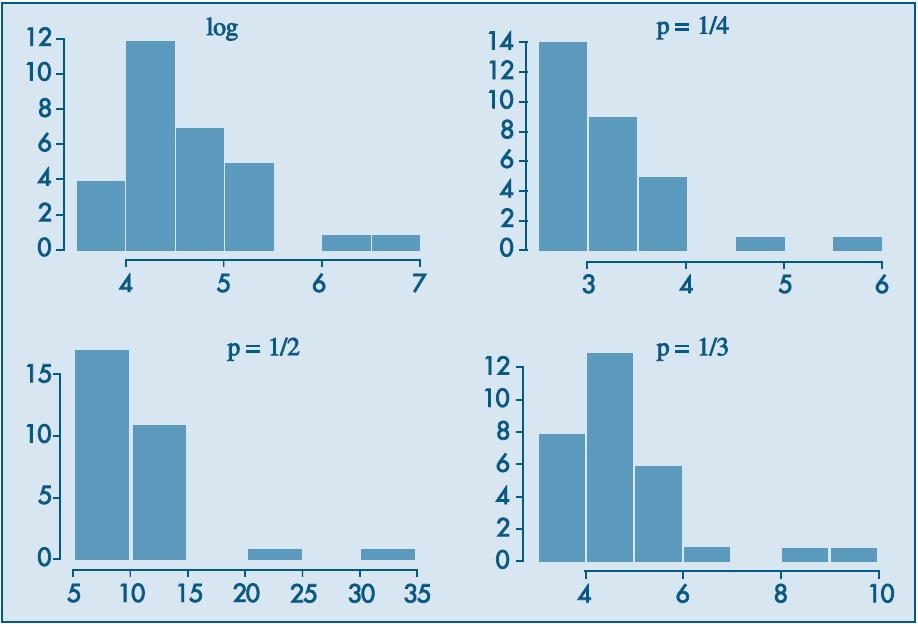
\includegraphics[height=0.4\textwidth,width=15cm]{Fig11}
    \caption{Exemplo de Histogramas para dados transformados (\cite{Morettin09}).}
    \label{Fig101_ex}
  \end{figure}
\end{frame}

\begin{frame}{}
\frametitle{Referências Bibliográficas}
\bibliography{bibliografia}
\end{frame}

\end{document} 
